\documentclass[runningheads,14pt,a4paper,openany]{book}

% Добавя възможност за сензитивни хипер-връзки в самия документ.
\usepackage[linktocpage=true,bookmarks=false]{hyperref}
\usepackage{nameref}
\usepackage[utf8x]{inputenc}
\usepackage[english,bulgarian]{babel}
\usepackage{url}
\usepackage{lipsum}
% Според изискванията на ИИКТ-БАН не бива да има номерация на страниците в ръкописа.
%\usepackage{nopageno}
\usepackage{shorttoc}
\usepackage[pdftex]{graphicx}
% Директория в която се намират изображенията.
\graphicspath{{images/}}
\usepackage{array,arydshln}
\usepackage{imakeidx}
\usepackage{placeins}
% Използва се за включване на кориците под формата на PDF файлове.
\usepackage{pdfpages}
% Служи за управление на заглавията.
\usepackage{fancyheadings}
%\usepackage{bookmark}

% Добавени от доц. Вера Ангелова.
%\usepackage{amsmath,amssymb,amsthm}
%\usepackage{longtable}
%\usepackage{pifont}   
%\usepackage{epsfig}
%\usepackage{tocloft}
%\usepackage{etoc}
%\usepackage{wasysym}
%\usepackage{eurosym}
%\usepackage{slashbox}
%\usepackage{soul}
%\usepackage{enumitem}
%\usepackage{mathcomp}
%\usepackage{epstopdf}
%\usepackage{latexsym}
%\usepackage{eucal}
%\usepackage{mathrsfs}

\textheight 22.8cm
\textwidth 17cm
\oddsidemargin -0.54cm
\evensidemargin -0.54cm
\topmargin 1.5cm

\parskip=0.2cm
\parindent=20pt
\flushbottom

% Премахва подчертаващата линия в заглавните части.
\renewcommand{\headrulewidth}{0pt}

\selectlanguage{bulgarian}

\lhead[\thepage \quad Тодор Балабанов \quad \hfill]{}
\chead{}
\rhead[]{\hfill Apache OpenOffice Calc за корпоративна употреба \quad \thepage }
\lfoot{}
\cfoot[\em Лекции по компютърни науки и технологии на ИИКТ - БАН, № *, 20**]{\em Лекции по компютърни науки и технологии на ИИКТ - БАН, № *, 20**} 
\rfoot{}

\onecolumn
\makeindex[columns=1, title=Азбучен указател, intoc]

\begin{document}

\def\ql{\textquotedblleft}\def\qr{\textquotedblright}


\includepdf[pages={1,2}]{images/front}
\thispagestyle{empty}

\voffset =-1truecm

% Използва се за номерация на страниците.
\renewcommand{\thepage}{\roman{page}}

\setcounter{page}{-1}
\thispagestyle{empty}
\pagestyle{empty}
\thispagestyle{empty}

% Тук стои таблицата със съдържанието, което се генерира от названието на главите.
\newpage
\thispagestyle{empty}
\pagestyle{empty}
\shorttoc{Теми}{0}
\thispagestyle{empty}
\pagestyle{empty}

% Тук стои таблицата със съдържанието, което се генерира от названието на главите и названието на секциите в тях.
\newpage
\thispagestyle{empty}
\pagestyle{empty}
\thispagestyle{empty}
\tableofcontents
\thispagestyle{empty}
\pagestyle{empty}

% Списък с фигурите.
\newpage
\listoffigures
\addcontentsline{toc}{chapter}{Списък на фигурите}

% Списък с таблиците. 
\newpage
\listoftables
\addcontentsline{toc}{chapter}{Списък с таблиците}

\newpage
\addcontentsline{toc}{chapter}{Предговор}
\chapter*{Предговор}
\pagenumbering{arabic}
\setcounter{page}{1}
\pagestyle{fancyplain}

Calc е софтуер за електронни таблици, който влиза в състава на програмния продукт Apache OpenOffice. По настояще Calc се разпространява като софтуер с отворен код под два основни лиценза – SISSL и GNU LGPL. Calc основно се използва за създаване и оформление на таблици, изчисления, обработка и анализ на данни, както и за графично представяне на резултатите от обработката. Учебното помагало е предназначено за офис работници (ръководители, мениджъри, секретари, финансови анализатори и други), ученици и студенти. 

Учебното помагало представя графичния интерфейс на Calc. Демонстрирате се основните елементи на потребителския интерфейс и начина за работа с тях. Засягат се темите за работа с файловата система на операционната система. Отделя се внимание за начина по който Calc зарежда и съхранява файлове, както и за възможностите да обработва информация от алтернативни софтуерни продукти за електронни таблици. Засягат се въпросите за работа с документи и списъчна информация. Набляга се на въвеждането, манипулирането и обработването на таблична информация. Значително внимание се отделя на възможностите за изчисления в Calc. Акцент е работата с формули, организиране на изчисленията и използването на наличните в Calc математически функции. Допълнително внимание е отделено за форматирането на таблиците и графичното им оформление. Разглеждат се възможностите за сортиране и филтриране на данни. Демонстрират се основни принципи за защита на информацията. Представя се работа с диаграми от различни видове – създаване, редакция, оформление и настройки. Засягат се темите за оформление на печатните страници и разпечатването на принтер. 

Глава 1 - \nameref{chapter01}: Представя процеса по изтегляне, инсталиране и стартиране на програмния продукт.

Глава 2 - \nameref{chapter02}: Запознава с основните елементи на графичния потребителски интерфейс в основния работен прозорец.


\newpage
\chapter{Инсталация и стартиране}
\label{chapter01}

\newpage
\chapter{Работа в основния прозорец}
\label{chapter02}

На различните операционни системи графичният потребителски интерфейс\index{потребителски интерфейс} изглежда по леко различен начин, но основните функционалности са едни и същи (Фиг. \ref{figure0007}).

\section{Основен работен екран}

\begin{figure}[h!]
  \centering
  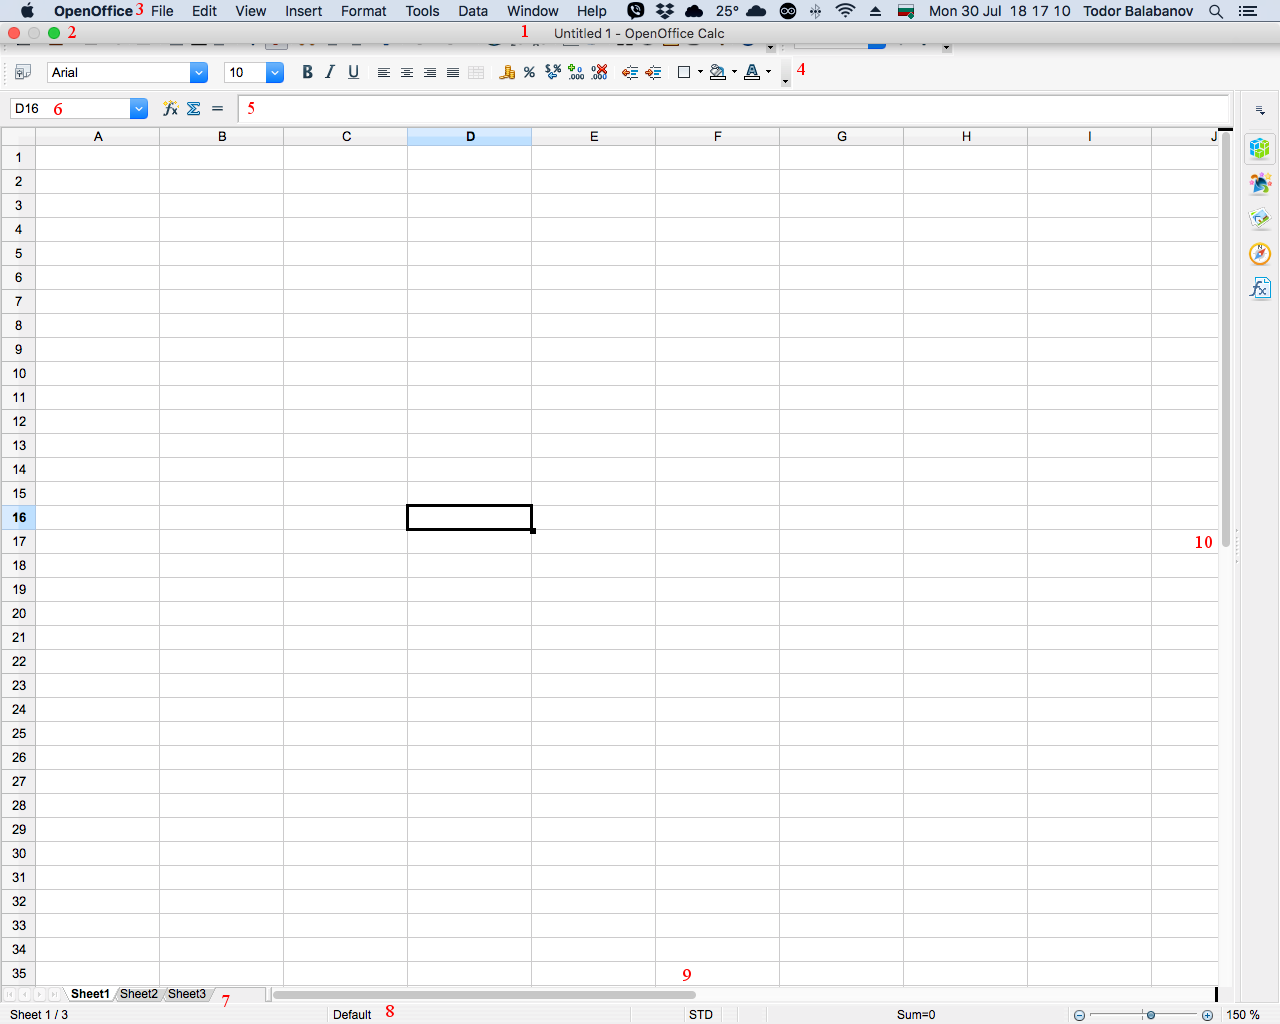
\includegraphics[width=1.0\linewidth]{pic0007}
  \caption{Заглавна лента с менюта}
\label{figure0007}
\end{figure}
\FloatBarrier

Най-отгоре (Фиг. \ref{figure0007} - 1), стои заглавната лента\index{заглавна лента} в която е изписано името на файла с който се работи. Когато не е зареден вече съществуващ файл, за име на файл се използва служебна комбинация от букви и цифри. В лявата част на заглавната лента се намират бутоните за управление на прозореца\index{управление на прозореца} (Фиг. \ref{figure0007} – 2). Над заглавната лента се намира лентата с менютата\index{лента с менюта} (Фиг. \ref{figure0007} – 3). На различните операционни системи лентата с менютата може да стои на различно място спрямо заглавната лента. Под заглавната лента стои панелът с инструментите (Фиг. \ref{figure0007} – 4). Под панела с инструментите стои панелът за въвеждане на формули\index{въвеждане на формули} (Фиг. \ref{figure0007} – 5). От ляво на панела за формули стои панела за въвеждане на адрес, за клетка или регион от клетки\index{адресиране на клетки} (Фиг. \ref{figure0007} – 6). Долу, в ляво са разположение работните листи\index{работни листи} (Фиг. \ref{figure0007} – 7). От дясно на работните листи се намира лентата за състоянието\index{лента на състоянието} на документа (Фиг. \ref{figure0007} – 8). Хоризонталният (Фиг. \ref{figure0007} – 9) и вертикалният (Фиг. \ref{figure0007} – 10) плъзгачи служат за преглеждане на работната област, когато тя надвишава видимата област от екрана. 

\section{Менюта}

Менютата\index{менюта} на програмния продукт съдържат команди\index{команди}, които са групирани според действията за които са предназначени (Фиг. \ref{figure0008}). В менюто OpenOffice са организирани командите, които се отнасят до функционалности в целия пакет, а не само в модула Calc. В менюто File са разположени команди за работа с файлове (зареждане, съхраняване, експортиране и други). Менюто Edit съдържа команди за редактиране на информация, като копиране, поставяне и други. Менюто View дава различни възможности за визуализация на активния документ. Менюто Insert дава възможности за вмъкване на различни обекти в работния документ. Менюто Format дава възможности за форматиране на различни обекти или части от документа. В менюто Tools са поместени инструменти за по-специфична обработка, като речници за езика, модули за проверка на граматиката и правописа, команди за работа с макроси и други. В менюто Data са поместени команди за обработка на данните, като сортиране или филтриране. Менюто Window дава възможности за работа с активните прозорци. И последното меню Help служи за допълнителна информация относно цялостната работа на системата. 

\begin{figure}[h!]
  \centering
  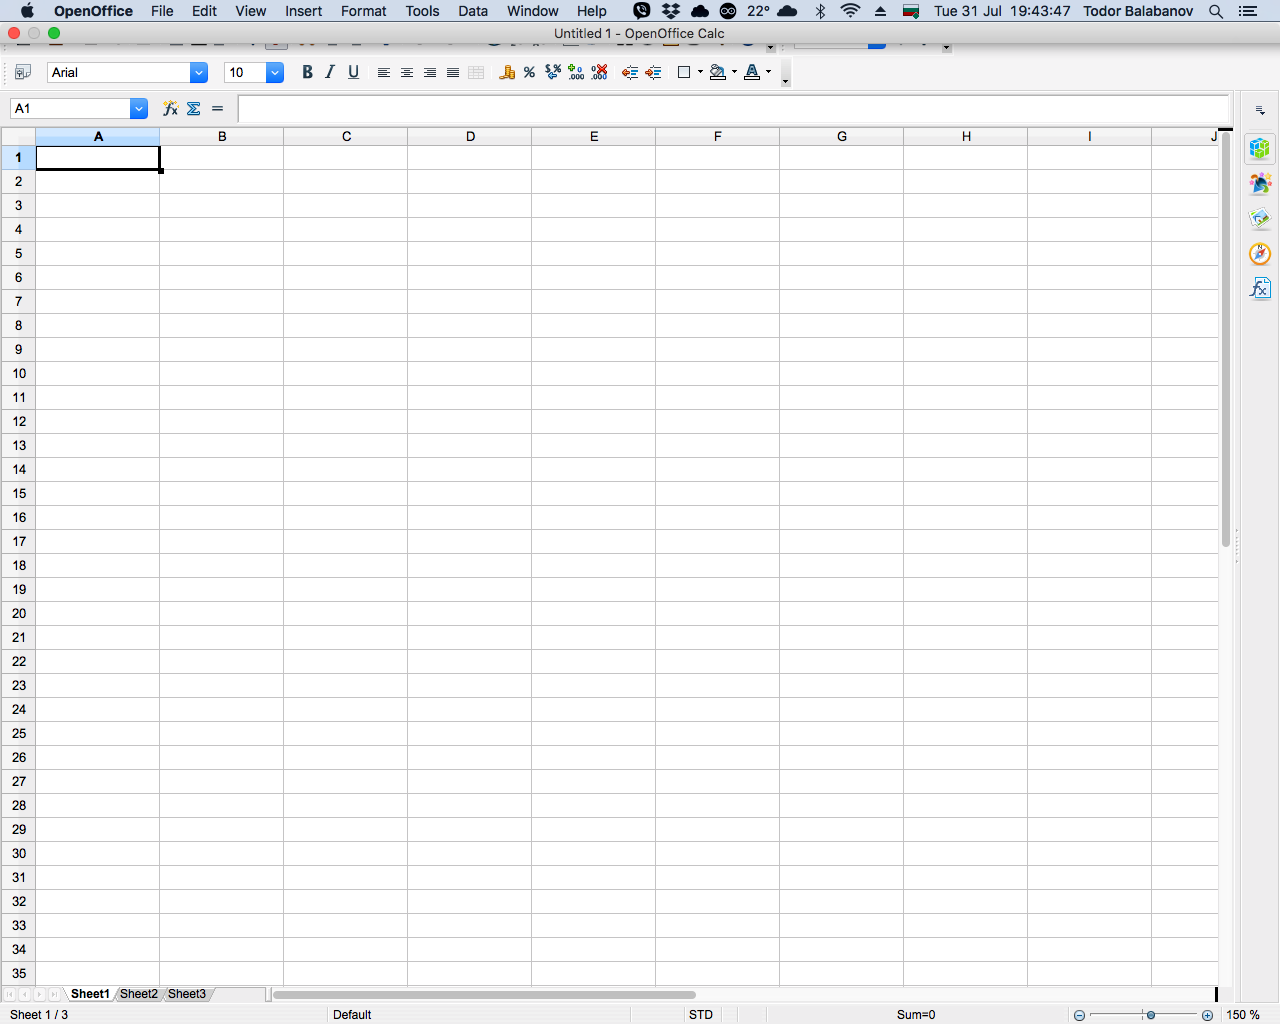
\includegraphics[width=1.0\linewidth]{pic0008}
  \caption{Главна група менюта}
\label{figure0008}
\end{figure}
\FloatBarrier

За да се изпълни команда от меню системата, то първо с мишката трябва да се избере конкретно меню, а след това опция в самото меню. Не всички команди по менютата са винаги достъпни. Това е така, защото някои от командите са контекстно зависими и имат смисъл само при определени условия. Недостъпните команди са изобразени в бледи цветове. С цел ускоряването на работата с програмния продукт, някои от командите в меню системата позволяват извикване с бърза клавишна комбинация. Разбира се, тези клавишни комбинации може да се различават в определена степен на различните операционни системи. Някои команди в меню системата от своя страна също представляват менюта\index{под менюта} и са обозначени със стрелка от дясно на названието им. При избора на тези команди се отваря допълнително меню, което на свой ред дава възможност за избор от списък команди (Фиг. \ref{figure0009}). 

\begin{figure}[h!]
  \centering
  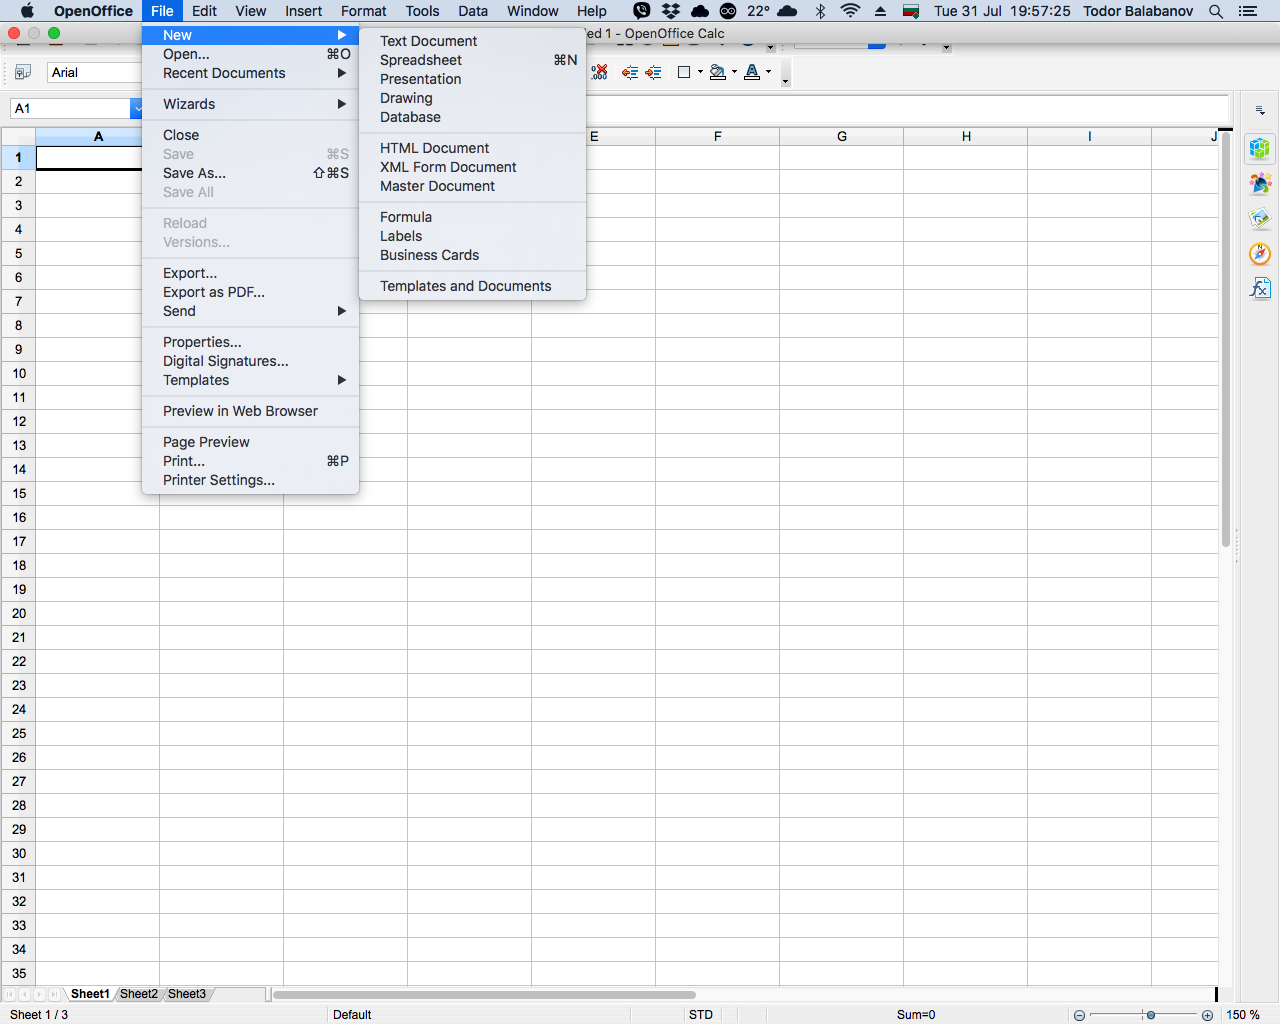
\includegraphics[width=1.0\linewidth]{pic0009}
  \caption{Под меню в основно меню}
\label{figure0009}
\end{figure}
\FloatBarrier

\section{Палитра с инструменти}

Палитрите с инструменти са организирани под лентата с менютата и също са групирани в панели. Палитрите с инструменти съдържат бутони за бързо изпълнение на най-често използваните команди. Както менютата, така и палитрите с инструменти подлежат на настройване от опциите на програмния продукт. Тези възможности дават свобода на потребителя да организира максимално ефективно виртуалното си работно пространство. Някои палитри с инструменти не са често използвани (примерно палитрата с инструменти за рисуване) и поради тази причина не са видими в основния екран. Палитрите, които не са видими биват активирани, когато се работи с клетки или обекти за които са предназначени. Повечето палитри с инструменти са прикачени за някои от ръбовете на основния прозорец, но е възможно палитрите да бъдат откачени и да имат свой самостоятелен мини-прозорец. 

\begin{figure}[h!]
  \centering
  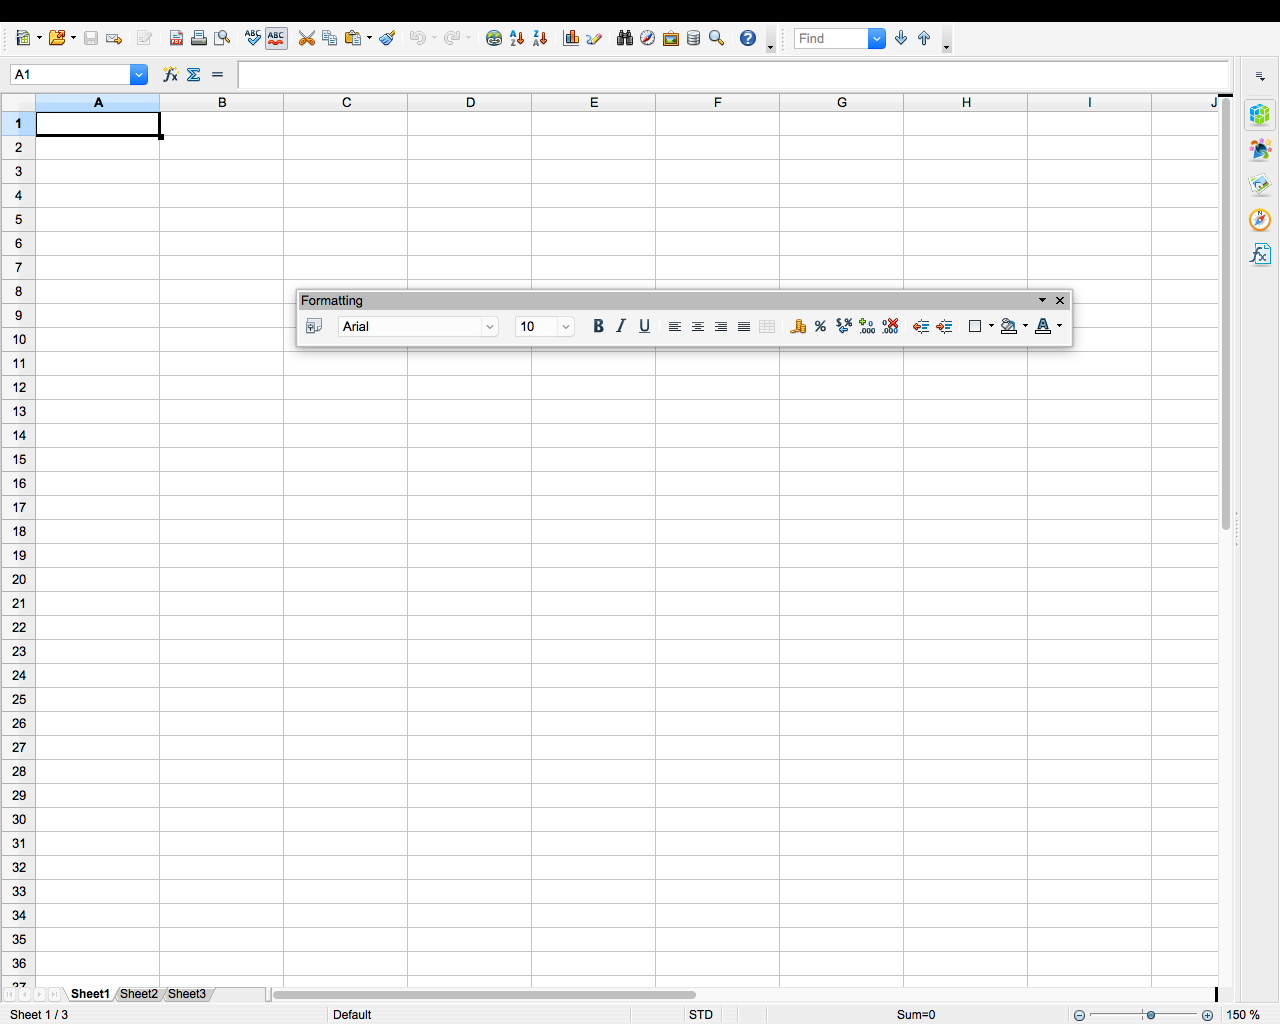
\includegraphics[width=1.0\linewidth]{pic0010}
  \caption{Свободно плаваща палитра с инструменти}
\label{figure0010}
\end{figure}
\FloatBarrier


\newpage
\addcontentsline{toc}{chapter}{Заключение}
\chapter*{Заключение}


% Списък с използвана литература и източници на информация.
\newpage
\begin{thebibliography}{99}
\addcontentsline{toc}{chapter}{Библиография}
\end{thebibliography}

% Азбучен указател на използваните термини.
\newpage
\printindex

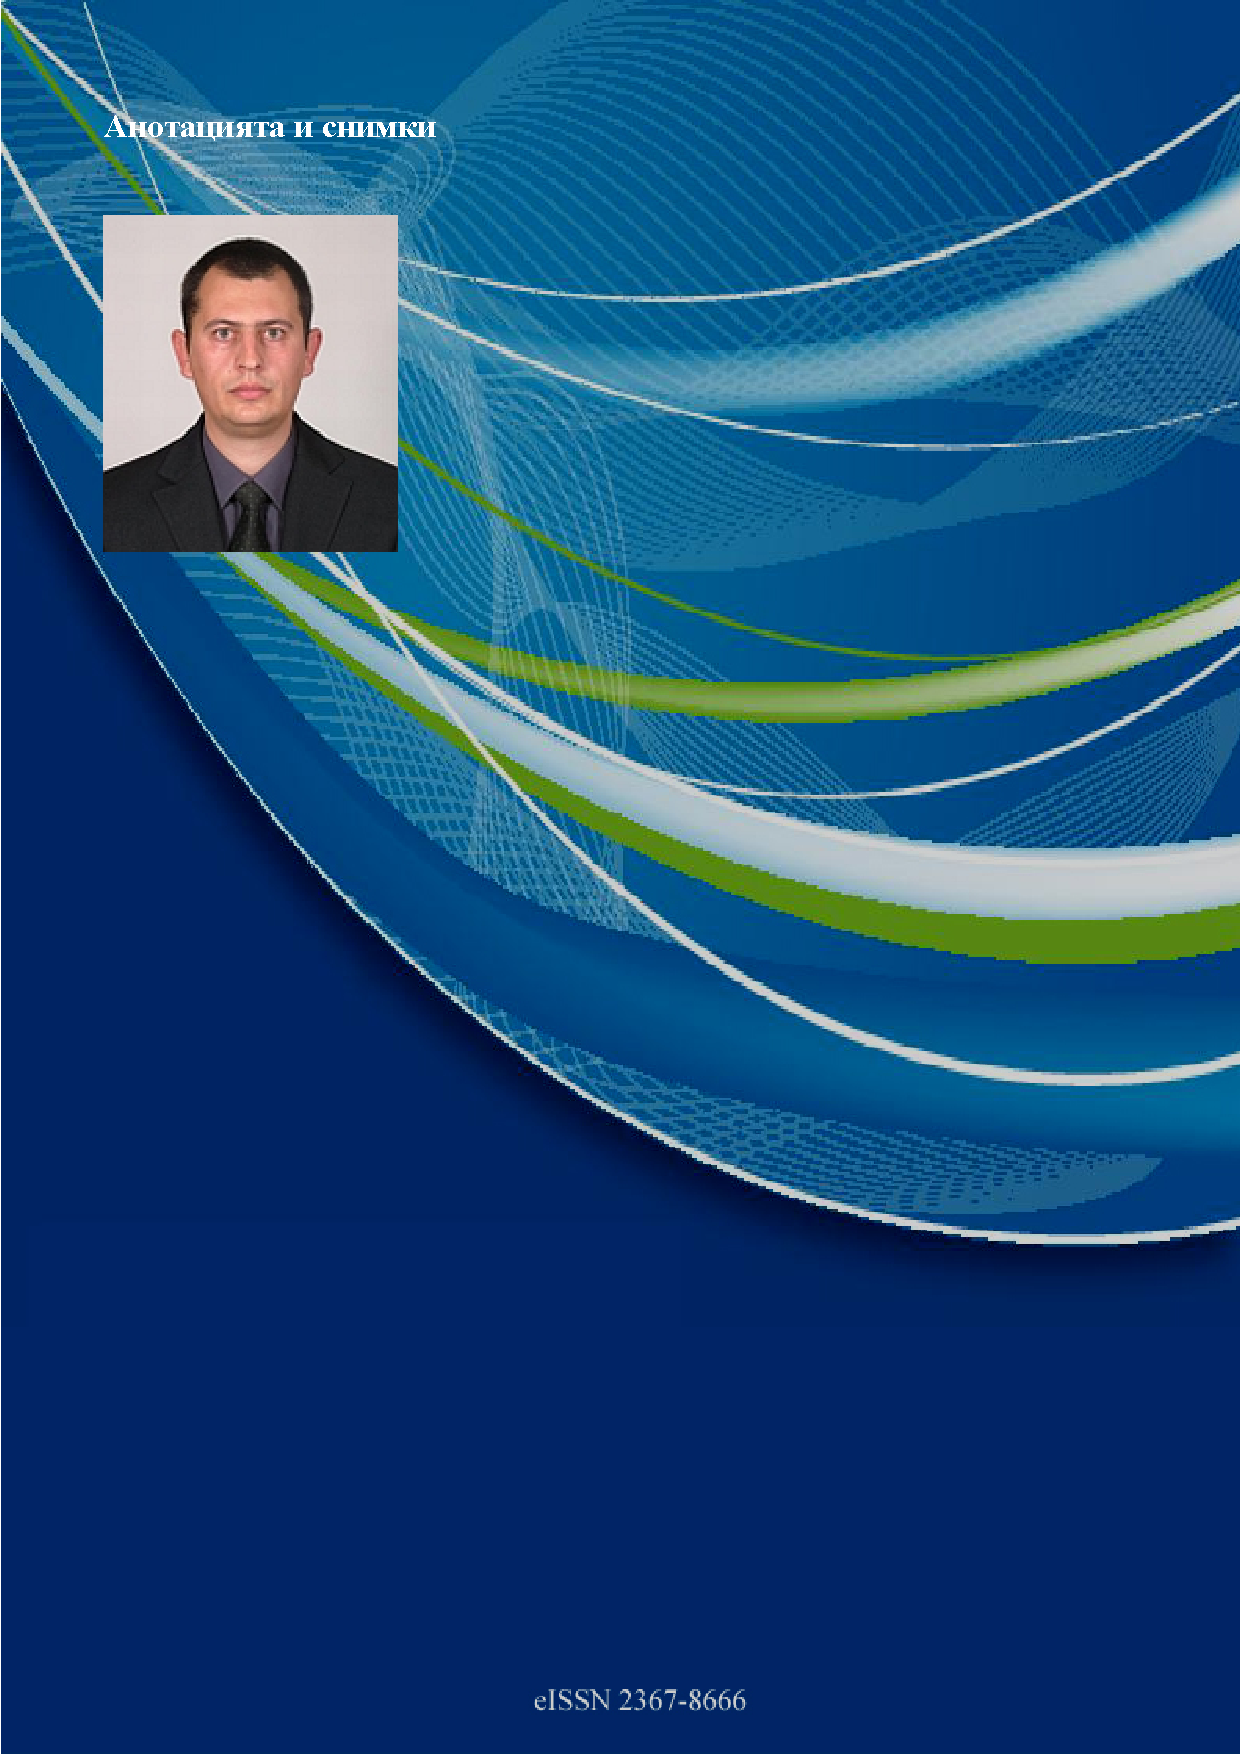
\includepdf[pages=-,height=320mm]{images/back}
\end{document}
